

\documentclass[SPC-MASTER.tex]{subfiles}
\begin{document}
\section*{Operating Characteristic (OC) Curves}
\begin{itemize}
\item A common supplementary plot to standard quality control charts is the so-called operating characteristic or OC curve (see example below). One question that comes to mind when using standard variable or attribute charts is how sensitive is the current quality control procedure? Put in more specific terms, how likely is it that you will not find a sample (e.g., mean in an X-bar chart) outside the control limits (i.e., accept the production process as "in control"), when, in fact, it has shifted by a certain amount? 

\item This probability is usually referred to as the  (beta) error probability, that is, the probability of erroneously accepting a process (mean, mean proportion, mean rate defectives, etc.) as being "in control." 

\item Note that operating characteristic curves pertain to the false-acceptance probability using the sample-outside-of- control-limits criterion only, and not the runs tests described earlier.


\item Operating characteristic curves are extremely useful for exploring the power of our quality control procedure. The actual decision concerning sample sizes should depend not only on the cost of implementing the plan (e.g., cost per item sampled), but also on the costs resulting from not detecting quality problems. The OC curve allows the engineer to estimate the probabilities of not detecting shifts of certain sizes in the production quality.
\end{itemize}

\subsubsection*{pistonrings Data}
\begin{framed}
\begin{verbatim}
#library(qcc)
data(pistonrings); attach(pistonrings);

diameter <- qcc.groups(diameter, sample)
beta <- oc.curves.xbar(qcc(diameter, type="xbar", nsigmas=3, plot=FALSE))
print(round(beta, digits=4))

# or to identify points on the plot use
## Not run: oc.curves.xbar(qcc(diameter, 
    type="xbar", nsigmas=3, plot=FALSE), identify=TRUE)

detach(pistonrings)
\end{verbatim}
\end{framed}

\begin{figure}
\centering
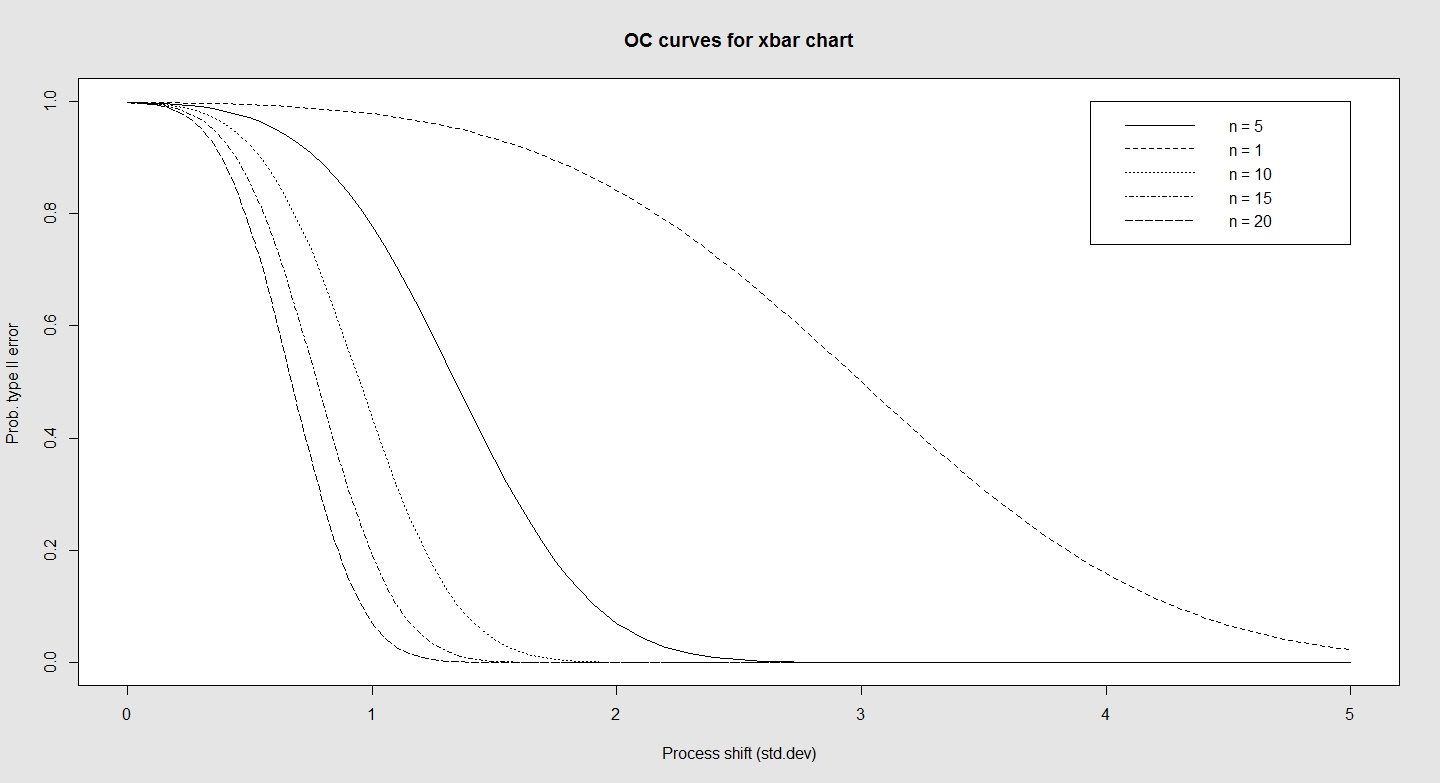
\includegraphics[width=0.7\linewidth]{images/OCpistonrings}
\caption{}
\label{fig:OCpistonrings}
\end{figure}

%======================================================================================%
\end{document}
